\begin{figure}
	\tikzsetnextfilename{zeeman-normale}
	\centering
	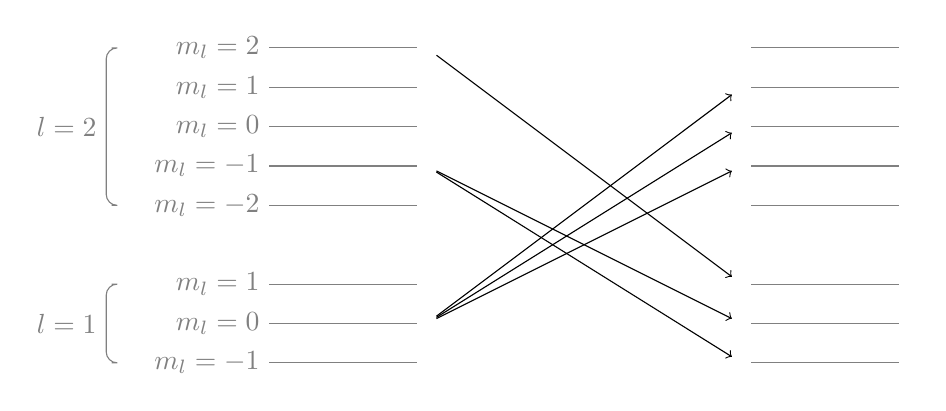
\begin{tikzpicture}
		% Sinistra
		\node (l1-1) at (-2,-1.5){};
		\node (l10)  at (-2,-1)  {};
		\node (l11)  at (-2,-0.5){};
		\node (l2-2) at (-2,0.5) {};
		\node (l2-1) at (-2,1)   {};
		\node (l20)  at (-2,1.5) {};
		\node (l21)  at (-2,2)   {};
		\node (l22)  at (-2,2.5) {};
		% Destra
		\node (r1-1) at (2,-1.5){};
		\node (r10)  at (2,-1)  {};
		\node (r11)  at (2,-0.5){};
		\node (r2-2) at (2,0.5) {};
		\node (r2-1) at (2,1)   {};
		\node (r20)  at (2,1.5) {};
		\node (r21)  at (2,2)   {};
		\node (r22)  at (2,2.5) {};
		% Raggruppamento delle linee con stesso n. quantico l
		\draw[rounded corners,black!50!white] (l1-1) ++(-4,0) -- ++(-2pt,0) to node[left]{$l=1$} ++(0,1) -- ++(2pt,0);
		\draw[rounded corners,black!50!white] (l2-2) ++(-4,0) -- ++(-2pt,0) to node[left]{$l=2$} ++(0,2) -- ++(2pt,0);
		% Linee spettrali non perturbate
		\draw[black!50!white] (l1-1) to +(-2,0) node[left]{$m_l=-1$};
		\draw[black!50!white] (l10)  to +(-2,0) node[left]{$m_l=0$};
		\draw[black!50!white] (l11)  to +(-2,0) node[left]{$m_l=1$};
		\draw[black!50!white] (l2-2) to +(-2,0) node[left]{$m_l=-2$};
		\draw[black!50!white] (l2-1) to +(-2,0) node[left]{$m_l=-1$};
		\draw[black!50!white] (l20)  to +(-2,0) node[left]{$m_l=0$};
		\draw[black!50!white] (l21)  to +(-2,0) node[left]{$m_l=1$};
		\draw[black!50!white] (l22)  to +(-2,0) node[left]{$m_l=2$};
		% Linee spettrali perturbate
		\draw[black!50!white] (r1-1) to +(2,0) node[right]{};
		\draw[black!50!white] (r10)  to +(2,0) node[right]{};
		\draw[black!50!white] (r11)  to +(2,0) node[right]{};
		\draw[black!50!white] (r2-2) to +(2,0) node[right]{};
		\draw[black!50!white] (r2-1) to +(2,0) node[right]{};
		\draw[black!50!white] (r20)  to +(2,0) node[right]{};
		\draw[black!50!white] (r21)  to +(2,0) node[right]{};
		\draw[black!50!white] (r22)  to +(2,0) node[right]{};
		% Frecce per indicare le transizioni tra i livelli
		\draw[thin,black,->] (l22) -- (r11);

		\draw[thin,black,->] (l2-1) -- (r10);
		\draw[thin,black,->] (l2-1) -- (r1-1);

		\draw[thin,black,->] (l10) -- (r21);
		\draw[thin,black,->] (l10) -- (r20);
		\draw[thin,black,->] (l10) -- (r2-1);
	\end{tikzpicture}
	\caption{Esempio della divisione di alcune linee spettrali dovuta all'effetto Zeeman normale.}
	\label{fig:zeeman-normale}
\end{figure}
